%% joser_template.tex
%% V1
%% 2008/12/15
%% by Davide Brugali
%% This is a skeleton file demonstrating the use of joser1.cls
%% with a JOSER paper
%%
%% This file is a modified version of bare_jrnl_compsoc.tex V1.3
%% by Michael Shell for IEEE CS journal papers
%% http://www.michaelshell.org/
%%
%%*************************************************************************
%% Legal Notice:
%% This code is offered as-is without any warranty either expressed or
%% implied; without even the implied warranty of MERCHANTABILITY or
%% FITNESS FOR A PARTICULAR PURPOSE!
%% User assumes all risk.
%% In no event shall JOSER or any contributor to this code be liable for
%% any damages or losses, including, but not limited to, incidental,
%% consequential, or any other damages, resulting from the use or misuse
%% of any information contained here.
%%
%% This work is distributed under the LaTeX Project Public License (LPPL)
%% ( http://www.latex-project.org/ ) version 1.3, and may be freely used,
%% distributed and modified. A copy of the LPPL, version 1.3, is included
%% in the base LaTeX documentation of all distributions of LaTeX released
%% 2003/12/01 or later.
%% Retain all contribution notices and credits.
%% ** Modified files should be clearly indicated as such, including  **
%% ** renaming them and changing author support contact information. **
%%
%%*************************************************************************

% Fixes by Dave
\setlength{\paperheight}{11in}
\PassOptionsToPackage{pdfpagelabels=false}{hyperref} 



\documentclass[10pt,journal,compsoc]{joser1}

% *** GRAPHICS RELATED PACKAGES ***
%
\ifCLASSINFOpdf
   \usepackage[pdftex]{graphicx}
\else
   \usepackage[dvips]{graphicx}
\fi

%%%%%%%%%%%%%%%%%%%%%%%%%%%%%%%%%%%%%%%%%%%%%%%%%%%%%%%%%%%%%%%%%%%%%%%
%%%%%%%%%%%%%%%%%%%%%%% will be inserted by the editor %%%%%%%%%%%%%%%%
%%%%%%%%%%%%%%%%%%%%%%%%%%%%%%%%%%%%%%%%%%%%%%%%%%%%%%%%%%%%%%%%%%%%%%%
\journalnumber{1}                       %will be inserted by the editor
\journalvolume{1}                       %will be inserted by the editor
\journalmonth{September}                %will be inserted by the editor
\journalyear{2013}                      %will be inserted by the editor
\articlefirstpage{1}                  %will be inserted by the editor
\articlelastpage{10}                   %will be inserted by the editor
\setcounter{page}{1}                  %will be inserted by the editor
%%%%%%%%%%%%%%%%%%%%%%%%%%%%%%%%%%%%%%%%%%%%%%%%%%%%%%%%%%%%%%%%%%%%%%%

\copyrightauthor{D. Coleman, I. Sucan, S. Chitta, N. Correll}
\headoddname{D. COLEMAN et al./ Reducing the Barrier to Entry of Complex Robotic Software}%

% correct bad hyphenation here
\hyphenation{op-tical net-works semi-conduc-tor}


\begin{document}
% paper title
\title{Reducing the Barrier to Entry of \\\vskip 0.3\baselineskip Complex Robotic Software}

\author{
David COLEMAN$^{1}$
\qquad
Ioan SUCAN$^{2}$
\qquad
Sachin CHITTA$^{3}$
\qquad
Nikolaus CORRELL$^{1}$

%%%%%%%%%%%%%%%%%%%%%%%%%%%%%%%%%%%%%%%%%%%%%%%%%%%%%%%%%%%%%%%%%%%%%%%
%%%%%%%%%%%%%%%%%%%%%%% will be inserted by the editor %%%%%%%%%%%%%%%%
%%%%%%%%%%%%%%%%%%%%%%%%%%%%%%%%%%%%%%%%%%%%%%%%%%%%%%%%%%%%%%%%%%%%%%%
\thanks{{\bf Regular paper} -- Manuscript received April 19, 2009;
revised July 11, 2009.}
%%%%%%%%%%%%%%%%%%%%%%%%%%%%%%%%%%%%%%%%%%%%%%%%%%%%%%%%%%%%%%%%%%%%%%%


\IEEEcompsocitemizethanks{\IEEEcompsocthanksitem This work was mostly performed while Coleman, Sucan, and Chitta were at Willow Garage, Inc.
.\protect\\

\IEEEcompsocthanksitem Authors retain copyright to their papers
and grant JOSER unlimited rights to publish the paper
electronically and in hard copy. Use
of the article is permitted as long as the author(s) and the journal are properly
acknowledged.}

} % end author

\address{
$^1$ Dept. of Computer Science, University of Colorado at Boulder, 430 UCB, Boulder, CO 80309\\
$^2$ Willow Garage, Inc., 68 Willow Road, Menlo Park, CA 94025\\
$^3$ SRI International, 333 Ravenswood Avenue, Menlo Park, CA 94025
}


% The paper headers
\markboth

\IEEEcompsoctitleabstractindextext{%
\begin{abstract}
Developing robot-agnostic software frameworks involves synthesizing disparate fields of robotic theory and software engineering while simultaneously accounting for a large variability in hardware designs and control paradigms. As the capabilities of robotic software frameworks increases, the setup difficulty and learning curve to new users also increases. If the entry barriers for configuring and using the software on robots is too high, even the most powerful of frameworks are useless. A growing need exists in robotic software engineering to aid users in getting started with, and customizing, the provided components as necessary for particular robotic applications. In this paper a case study is presented for the best practices found for lowering the barrier of entry of the MoveIt! motion planning framework that allows users to 1) quickly get basic motion planning functionality with minimal initial setup, 2) automate its configuration and optimization, and 3) easily customize its components. A graphical 
interface that assists the user in configuring MoveIt! is the cornerstone of our approach, together with a standardized robot model for input, automatically generated robot-specific configuration files, and a plugin-based architecture for extensibility. These best practices are summarized into a set of \textit{barrier to entry design principles} applicable to other robot software. The approaches for lowering the entry barrier are evaluated by usage statistics, a user survey, and compared against our design objectives for their effectiveness to users.\\
TODO: abstract limit is 200 words. ''300 words are also acceptable.''
\end{abstract}

\begin{IEEEkeywords}
Robotic Software Frameworks, Motion Planning, Barrier to Entry, Setup, Usability, MoveIt!
\end{IEEEkeywords}}

% make the title area
\maketitle


% ====================================================================
% ====================================================================
% Section
% ====================================================================
% ====================================================================
\section{Introduction}
% The very first letter is a 2 line initial drop letter followed by the rest of the first word in caps.
\IEEEPARstart{M}{anaging} {the increasing complexity of modern robotic software is a difficult engineering challenge faced by roboticists today. The size of the code bases of common open source robotic software frameworks such as ROS \cite{quigley2009ros}, MoveIt! \cite{moveit} and OROCOS \cite{bruyninckx2001open} continues to increase \cite{makarenko2007benefits}, and the required breadth of knowledge for understanding the deep stack of software from control drivers to high level planners is becoming more daunting. As it is beyond the capabilities for any one researcher to have the necessary domain knowledge for every aspect of a robot's tool chain, it is becoming increasingly necessary to assist users in the configuration, customization, and optimization of the various software components of a reusable robotic framework. 

The user interface design principles required in the emerging field of robotics software is similar to other more mature software engineering fields and much can be learned from them. There have been many examples of software, such as computer operating systems, that have historically required many installation and configuration steps. As those software fields matured, the entry to barriers have decreased and become easier for users to accomplish. Still, robotics software in general is unique in 1) the degree to which software interacts with hardware and real world environments, 2) the lack of maturity in the field results in many varying approaches for solving a problem, and 3) the long term desire to increase the autonomy of robotics systems. 

% ====================================================================
\subsection{Barriers to Entry}

The term \textit{barriers to entry} is used in the context of robotic software engineering to refer to the time, effort, and knowledge that a new user must invest in the integration of a software component with an arbitrary robot. This can include for example creating a virtual model of the robot's geometry and dynamics, customizing configuration files, choosing the fastest algorithmic approach for the application, and finding the best parameters for various algorithms.

Powerful robotics software generally requires many varying degrees of customization and optimization for any particular robot to operate properly. Choosing the right parameters for each utilized algorithm and software component typically involves expert human input using domain-specific knowledge. Many new users to a software package, particularly as robotics becomes more mainstream, will not have the breadth of knowledge to customize every aspect of the tool chain. When the knowledge of a new user is insufficient for the requirements of the software, the barriers to entry become insurmountable and the software unusable. One of the emerging requirements of robot agnostic frameworks is implementing mechanisms that will automatically setup and tune task pipelines for arbitrary robots.

Another motivation for lowering the barrier to entry of complex robotics software is the \textit{paradox of the active user}. This paradox explains a common observation in many user studies that \textit{users never read manuals} but start attempting to use the software immediately \cite{carroll1987interfacing}. A user's desire to quickly accomplish a task results in them skipping reading any provided documentation or gaining deeper understanding of the system and instead diving right into completing their task. The \textit{paradox} is that the user would actually save time in the long run if they learned more about the system before attempting to use it, but these studies showed that in reality people do not tend to invest time upfront into learning a new system.

Even experts in the area of the associated robotics software will become frustrated with robotics software if all initial attempts to setup and configure the framework fail and no progress is made. Most researchers and engineers typically do not have the time or ability to completely understand the entirety of robotics software before they start using it. It is very important for the initial experience with a piece of software be positive for the continued use of the software by the user.

% ====================================================================
\subsection{Benefits of Larger User Base}

The need to lower the barrier of entry is beneficial to the software itself in that it enables more users to utilize the framework. If the software framework is being sold for profit, the benefits of larger user base is obvious. If instead the software is a free open-source project, as most successful robotic frameworks currently are \cite{makarenko2007benefits}, lowering the barrier to entry is very beneficial in that it creates the \textit{critical mass of skilled contributors} that has been shown to make open source projects successful \cite{bruyninckx2001open}. As the number of users increases, the speed in which bugs are identified and fixed increases \cite{schmidt1999software}. It is also typically hoped that development contributions to the code base increases, though this correlation is not as strong \cite{schmidt1999software}. One of the key strengths of a larger community for an open source project is increased participation of users assisting with quality assurance, documentation, and support \
cite{schmidt2001leveraging}.

Another benefit of lowering the barrier of entry is that it allows the robotics software to become an educational tool for robotics. Not only is the software accessible for academic research and industrial applications, but graduate, undergraduate, and even primary-level students can use it to learn some of the higher level concepts of robotic applications as has been demonstrated in \cite{correll2013one, moll2011teaching, guyot2011teaching}. This should not be the main focus of most robotics software, but a nice side effect.

Beyond the motivations of the success for an individual software project, broadening access to robotics software development increases the number of creative minds working on solving today's challenging robotics problems. Making robot programming more like mobile device programming and web development will perhaps increase the speed of innovation in robotics, similar to that experienced by phone apps and the Internet \cite{boudreau2012let}.

The target \textit{users} as used in this paper are engineers, scientists, students, and hobbyists with a general aptitude for software and robotics but who are not necessarily experts in either of those fields. The hope remains that human-robotic interaction for the general population in the future will be based on more natural methods, and that software configuration and GUIs are only necessary for the robot developers themselves.

% ====================================================================
\subsection{Difficulty of Robot Agnostic Software}

The software engineering challenges faced in making robot-agnostic code are hard - many shortcuts typical for single-robot software must be avoided, such as hard coding in domain-specific values and using heuristics applicable to only one hardware configuration. Accounting for all the edge cases of a robot's design requires many extra levels of abstraction. On top of these challenges, packaging up this reusable software into an easy to setup experience for end users requires creating many tools that automate the configuration of the software.

% ====================================================================
\subsection{Related Work}

There has been much written and developed to addressed the software engineering challenges of complex robotic frameworks, but typically the identified design goals have emphasized the need for features such as platform independence, scalability, real-time performance, software reuse, and distributed layouts \cite{realtime_framework, collett2005player, kramer2007development}. In \cite{kramer2007development}'s survey of nine open source robotic development environments, a collection of metrics were used which included documentation and graphical user interfaces (GUI), but no mention was made of setup time, barrier to entry, or automated configuration. 

The importance of an open source robotics framework having a large number of researchers and engineers motivated to contribute code and documentation is emphasized in the OROCOS framework \cite{bruyninckx2001open}, which we emphatically agree with but take a step further by creating additional tools to encourage higher user adoption.
  
Human-robot interaction (HRI) has also been a popular area of research, but HRI's focus has been on the runtime behavior of robots and not on the difficulties of human users applying software frameworks to robot hardware \cite{hci_metrics, yancotaxonomy, goodrichseven}. In \cite{rescueRobots}, an effective user interface is presented for teleoperation of rescue robots, but no thought is given to making it robot agnostic or to its configuration. 

From the best of our knowledge, there has been no prior work on the difficulties of setting up and configuring robotics software.

% ====================================================================
\subsection{Contribution and Outline}

In this paper we will present best practice principles for lowering the barrier of entry to robotic software using the new MoveIt! Motion Planning Framework as our case study. In section \ref{sec::motion_planning} we will motivate the many software components that make motion planning frameworks a good example of the difficulties of complex robotics software and in section \ref{sec::moveit} we will introduce MoveIt! itself. In section \ref{sec::requirements} we explain the design principles used to address the user interface needs of robotics software. We then show how we have taken these principles and implemented them in MoveIt! to reduce the entry barriers in section \ref{sec::lowering_barriers}. In section \ref{sec::results} we will present the results of these implementations on the size of the user base and ease of adoption of the MoveIt! software framework. We will discuss our experiences and lessons learned in section \ref{sec::discussion} followed by our conclusion in section \ref{sec::conclusion}.

% ====================================================================
% ====================================================================
% Section
% ====================================================================
% ====================================================================
\section{Motion Planning Frameworks}
\label{sec::motion_planning}

Robotic motion planning is a maturing and central field in robotics \cite{moll2011teaching} that turns a high level task command into a series of discrete motions such that a robot can move within its environment. The typical use case considered in this paper is the problem of controlling a robotic arm from one configuration to another while taking into account various constraints.

The software development of a motion planning framework (MPF) is challenging and involves combining many disparate fields of robotics and software engineering \cite{perez2010roadmap}. We refer to the software as a \textit{framework} in this context because it abstracts the various components of motion planning into generic interfaces as discussed later.

One of the most important features of a framework for motion planning is providing the structures and classes to share common data between the different components. These basic data structures include a model of the robot, a method for maintaining a representation of the state of the robot during planning and execution, and a method for maintaining the environment as perceived by the robot's sensors (the ``planning scene'').

In addition to the common data structures, a MPF requires many different interacting software components, henceforth referred to as the \textit{planning components}. A high level diagram of the various planning components is shown in Figure \ref{fig:motionplanning_highlevel}. The planning component that actually performs motion planning includes one or more algorithms suited for solving the expected problems a robot will encounter. The field of motion planning is large and no one-size fits all solution exists yet, so a framework that is robot agnostic should likely include an assortment of algorithms and algorithm variants.

\begin{figure}[!t]
\centering
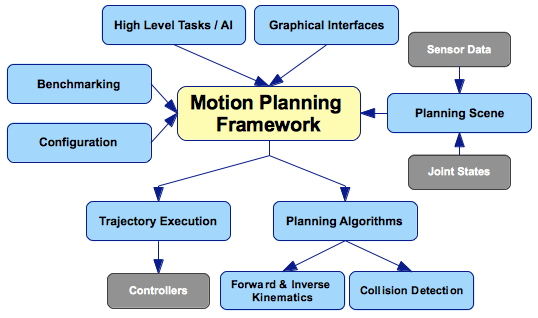
\includegraphics[width=3.4in]{images/motionplanning_highlevel}
\caption{High level diagram of various planning components in a MPF.}
\label{fig:motionplanning_highlevel}
\end{figure} 

Other planning components include a collision checking module that detects the potential intersection of geometric primitives and meshes in the planning scene and robot model. A forward kinematics solver is required to propagate the robot's geometry based on its joint positions, and an inverse kinematics solver is required when planning in the Cartesian space of the end effector for some of the planning techniques. Other potential constraints, such as joint/velocity/torque limits, and stability requirements, require additional components.

Secondary components must also be integrated into a powerful MPF. Depending on what configuration space a problem was solved in, a generated motion planning solution of position way points must be parameterized into a time-variant trajectory to be executed. A controller manager must decide the proper low level controllers for the necessary joints for each trajectory. A perception interface updates the planning scene with recognized objects from a perception pipeline as well as optional raw sensor data.

Higher level applications are built on top of these motion planning components to coordinate more complex tasks, such as pick and place routines. Other optional components of a MPF can include benchmarking tools, introspection and debug tools, as well as the user-facing GUI.

% ====================================================================
% Subsection
\subsection{Existing Motion Planning Software}
\label{sec::existing}

There exists many open source software projects for motion planning whose intent it is to provide a platform for testing novel path planning algorithms and other motion planning components. We will distinguish them differently from a motion planning \textit{framework} based on their exclusion of actual hardware perception and control. All offer varying degrees of modularity and all have a visualization window for viewing motion plans of 3D geometries. A brief review of them is presented here.

Both LaValle's Motion Strategy Library (MSL) \cite{lavallemsl}, 2000, and Latombe's Motion Planning Kit (MPK) TODO all citations in this section \cite{}, 2003 have scopes limited to only simulation so are not frameworks in our definition. The MSL is configured manually using 6 required files and up to 15 optional files, depending on the planning problem. It has a GUI for tweaking parameters and controlling the visualization of plans. The MPK is able to load robots with varying geometry without recompiling code, ad provides a scene format that is an extension of the Open Inventor format. It does not have a GUI but rather allows control through pure keyboard shortcuts. Neither MSL or MPK provide in assistance in setting up a new robot and have unclear documentation on this process.

The Karvaki Lab's Object-Oriented Programming System for Motion Planning (OOPSMP) \cite{}, 2008, is a predecessor to the Open Motion Planning Library (OMPL) \cite{}, 2010, both of which are collections of planning algorithms and components whose scope again falls short hardware execution and perception tasks. OOPSMP is XML based for configuration, scene definitions, and robot geometry. An additional SketchUp interface provides a quick way to build environments. It has some GUIs. OPMPL differs in its handling of environments and robots in that it abstracts that notion into a black box and instead only operates in various configuration spaces. It is intended to not be used stand alone but rather within a motion planning framework like MoveIt!, discussed later. Neither OOPSMP nor OMPL provide any tools or GUIs for configurations.

Diankov's OpenRave  \cite{}, 2010, is a fully featured motion planning framework with many high level capabilities, some GUIs, and the ability to connect to hardware controllers and sensors. It uses the Collada format \cite{collada}, as well as its own proprietary format, to define robots and environments. Its main interface is through simple python scripting and it utilizes a plugin interface to provide extensibility of the framework. It too falls short of providing easy to setup tools for new robots. 

Willow Garage's ROS Arm Navigation framework \cite{}, 2010, is the processor of MoveIt! and provides much of the same functionality of Moveit and OpenRave but also includes a Setup Wizard that provides a GUI for helping new users setup arbitrary robots into the framework. It was the inspiration for the Setup Assistant described later in this paper.

% ====================================================================
% Subsection
\subsection{MoveIt! Motion Planning Framework}
\label{sec::moveit}

MoveIt! is the primary motion planning framework in ROS and has been successfully integrated with many robots including the PR2 \cite{wyrobek2008towards}, Robotnaut \cite{ambrose2000robonaut}, and Atlas. It is a popular open source project developed initially at Willow Garage that aims to become the open standard for motion planning research and applications. MoveIt! is written entirely in C++ but also includes Python bindings for higher level scripting. It follows the principle of software reuse as advocated for robotics in \cite{makarenko2007benefits} of not tying itself exclusively to one robotic framework - in our case ROS - by creating a formal separation between core functionality and robotic framework-dependent aspects. 

By default MoveIt! is built on ROS and integrates the Open Motion Planning Library (OMPL) \cite{sucan2012the-open-motion-planning-library} for planning, the Fast Collision Library (FCL) \cite{fcl} for collision checking, and the OROCOS Kinematics and Dynamics Library (KDL) \cite{kdl} for forward and inverse kinematics. The ability to change these default planning components in discussed in section \ref{subsec:extensiblity}.

MoveIt!'s target application is for the control of an articulated rigid body robot in a wide range of environments. Although it has primarily been developed for single and dual arm manipulation, it can also be applied to non-holonomic vehicles, rotocraft and other configuration spaces. It is intended to be used in industrial, consumer, and research settings.

% ====================================================================
% ====================================================================
% Section
% ====================================================================
% ====================================================================
\section{Entry Barrier Design Principles}
\label{sec::requirements}

In designing the configuration process required to enable MoveIt! to work with many different types of robots, with almost any combination of planning components, several contending design principles for lowering the barrier of entry emerged. These requirements were drawn partially from standard HCI principles \cite{galitz2007essential}, from work on MoveIt!'s predecessor - the \textit{arm\_navigation} project, and from an iterative design process where feedback was gained from internal users at Willow Garage during development. We believe these \textit{entry barrier design principles} transcend motion planning and can be applied to most robotic software:

{\bf Immediate}: The amount of time required to accomplish the most primitive task expected from the robotic software component should be minimized. This is similar to the time-honored ``Hello World'' demo frequently used by programming languages and typical Quick Start guides in documentation. Immediacy is essential for the \textit{paradox of the active user} as it provides cursory feedback to the user that the software works and is worth investing further time.

{\bf Transparent}: The configuration steps being performed automatically for the user, and the underlying mechanisms utilized in the software components, should be as visible as possible. Transparency is important so that the user can later understand what parameters are specific to their robot and know how to customize the aspects they desire. Hiding too much of the setup process can lead the user user to being hindered in the future.

{\bf Intuitive}: The need to read accompanied documentation, and the amount of required documentation, should be minimized. A well designed user interface, be it graphical or command line, should be as intuitive as possible by following standard design patterns and providing interface context clues. An ideal GUI for configuration would not require any documentation for most users.

{\bf Reconfigurable}: The automatically generated parameters and default values for the initial setup of a robot should be easy to modify at a later time by the user. Typically these parameters and values are chosen to work for the largest number of robots possible, but are not optimal for any particular robot. Providing easy methods to reconfigure the initial setup is very important. 

{\bf Extensible}: The ability of the user to customize as many components and behaviors as possible within the reasonable scope of the software. Providing the means to extend the software with custom solutions for a particular application will make the software far more powerful and re-usable for varying use-cases. A typical solution for this is providing a plugin interface.

{\bf Documented}: The amount of reference material explaining how to use the software should be maximized for as many aspects and user levels as possible. Even the most intuitive software requires documentation for various aspects of the operation or modification of the software itself. Different types of documentation are needed for different users - for example developers and end users - though in robotics this is frequently the same. Documentation is arguably the most important factor in reducing the barrier to entry of new software \cite{forward2002relevance}.

Many of these principles have opposing objectives that require a trade off or balance be found between them. For example, the desire for transparency in the underlying mechanisms often leads to slower setup times (immediacy) and more complicated configuration steps (unintuitive). The need for extensibility of various components in the software often results in far more complicated software design as more abstraction is required, resulting in a less intuitive code base and difficult documentation. Nevertheless, compromises can be made between these principles that result in a superior user experience as will be demonstrated in the next section.

% ====================================================================
% ====================================================================
% Section
% ====================================================================
% ====================================================================
\section{Methods to Lower The Entry Barrier}
\label{sec::lowering_barriers}

One of the unique features of MoveIt! is the ratio of its power and features to the required setup time. A beginner to motion planning can take a model of their robot and with very little effort execute motion plans in a virtual environment. With a few additional steps of setting up the correct hardware interfaces, one can then execute the motion plans on actual robotic hardware.

The \textit{entry barrier design principles} discussed above were applied to MoveIt! to address the challenges faced for new users to this complex software framework. Developing these solutions required difficult software challenges be overcome as discussed in the following.

% ====================================================================
\subsection{Basic Motion Planning Out of the Box}

To address the entry barrier design principle of \textit{immediacy}, a streamlined ``Quick Start'' for MoveIt! was created that consists of a series of fairly trivial steps, relative to our target users. The most challenging of these steps - creating a \textit{robot model} - is not directly related to the configuration of MoveIt!, but rather is a prerequisite of using the software framework. Nevertheless, we will discuss this important prerequisite before preceding to the more directly-related configuration steps. 

{\bf Robot Model Format}: The robot model is the data structures and accompanying file format used to describe the three-dimensional geometric representation of the robot, its kinematics, as well as other properties relevant to robotics. These other properties can include the geometric visualization meshes, courser-grained collision geometry of the robot used for fast collision checking, joint limits, sensors, and dynamic properties such as mass, moments of inertia, and velocity limits. Often the robot's joints and links relationships are represented by a kinematic tree, though this approach is problematic when a robot has a closed chain. In our application, as well as most state of the art MPFs, we will restrict our definition of modeled robots to arbitrarily articulated rigid bodies. 

Extensible robotics software requires using a standardized format that can express the intricacies of varying hardware configurations. An additional design requirement for this standardized format is that it is \textit{intuitive} for users to setup. There are a few options for representing robots, and in MoveIt! it was accomplished by utilizing the human-readable XML schema provided by ROS for robot models - the Universal Robotic Description Format (URDF) \cite{urdf}. This data structure format can accept URDF-formatted files, as well as the industry standard Collada \cite{collada} format.

Creating a accurate model of a robot can be a difficult task. There already exists URDF models for many robots, so often users can avoid the problem. However, when a custom robot requires a new robot model, URDF was partially chosen because of the tools it provides to help with this task. There is a tool for verifying the validity of the XML, for visualizing it, and for converting a SolidWorks CAD model of a robot directly into URDF format. 

{\bf MoveIt! Setup Assistant}: The main facility that provides out of the box support for beginners is the MoveIt! Setup Assistant (SA). The SA is a GUI that steps new users though the initial configuration requirements of using a custom robot with the motion planning framework (Figure \ref{fig:setupassistant}). It accomplishes the task for the user of automatically generating all the many configuration files necessary for the initial operation of MoveIt!. These configurations include a self-collision matrix, planning group definitions, robot poses, end effector semantics, virtual joints list, and passive joints list. 

\begin{figure}[!t]
\centering
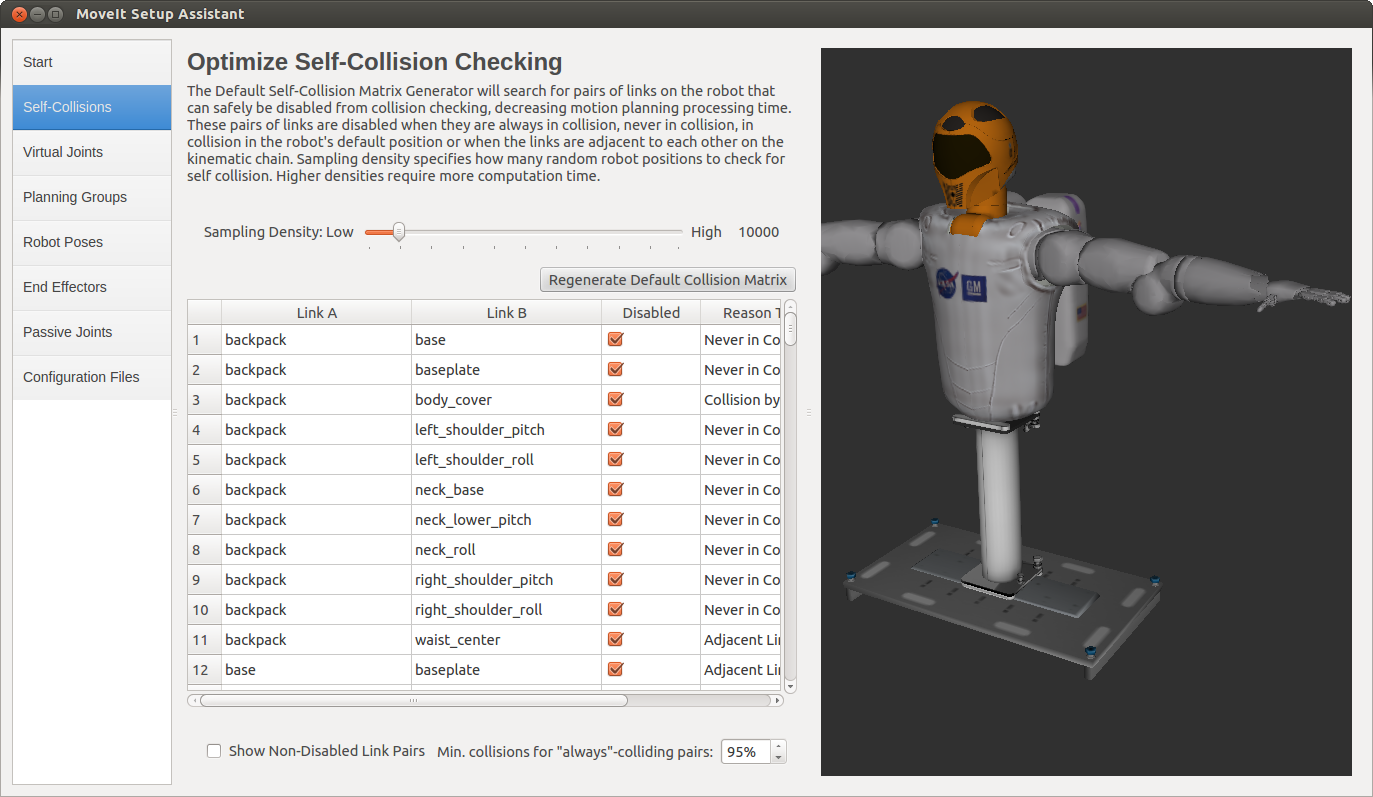
\includegraphics[width=3.4in]{images/setup_assistant}
\caption{MoveIt! Setup Assistant GUI with the NASA Robonaut loaded in the self-collision matrix screen.}
\label{fig:setupassistant}
\end{figure}

The GUI consists of 1) large navigation pane on the left that allows the user to move non-linearly through the setup process as needed, 2) the middle settings window that changes based on the current setup step being performed by the user, and 3) a right side visualization of the three dimensional model of the robot as it is being configured. The right side visualization increases the immediacy of results and transparency of the configuration by highlighting various links of the robot during configuration to visually confirm the actions of the user, as shown in Figure \ref{fig:setupassistant3}.

\begin{figure}[!t]
\centering
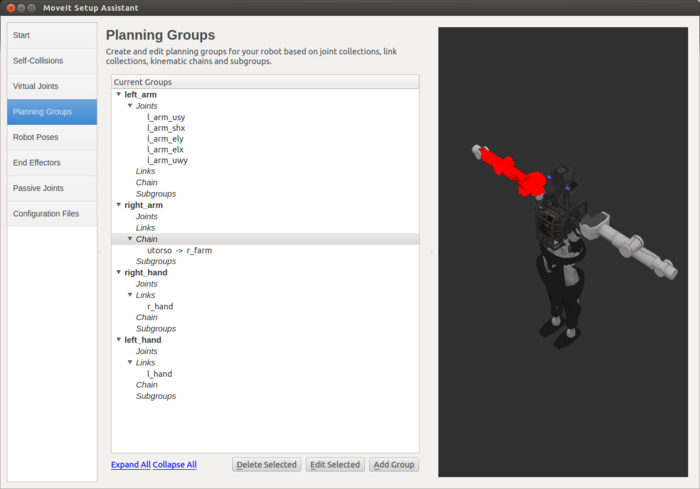
\includegraphics[width=3.4in]{images/setup_assistant3}
\caption{MoveIt! Setup Assistant GUI with the Atlas robot's left arm highlighted for user feedback on the planning groups screen.}
\label{fig:setupassistant3}	
\end{figure}

Using a properly formatted robot model file with the SA, MoveIt! can automatically accomplish many of the required tasks in a MPF. If one desired, the steps within the SA could almost entirely be automated themselves, but they have been kept manual so 1) increase transparency and 2) provide extensibility for edge cases and unusual customizations.

{\bf MoveIt! Motion Planning Visualization GUI}: The details of the automated configuration are left for the next section, but after the steps in the SA are completed a demo script that will automatically startup a visualization tool with the new robot loaded and ready to run motion planning algorithms in a non-physics based simulation. A typical demo task would be using the computer mouse to visually drag 3D interactive arrows situated on the robot's end effector from a start position to a goal position around some virtual obstacle. The demo can then quickly plan the arm in a collision free path around the obstacle and visualize the results within the GUI. 

This user interaction is accomplished with the MoveIt! Motion Planning Visualization (MMPV), an additional GUI that allows beginning users to learn and experiment with a large subset of the functionality provided by MoveIt! (Figure \ref{fig:motionrvizplugin}). While the long term goals of robotics is to provide more autonomous solutions to motion planning and human-robot interactions \cite{yancotaxonomy}, the MMPV fulfills the immediate needs of direct operation for testing and debugging the framework's capabilities easily. This interface is a vital component of MoveIt!'s strategy to provide immediate results for motion planning with a robot that does not require any custom coding. Once the user is comfortable with the basic feature set and functionality of MoveIt!, extensibility is provided via varying levels of code APIs for more direct, non-GUI, access to the robot's abilities.

\begin{figure}[!t]
\centering
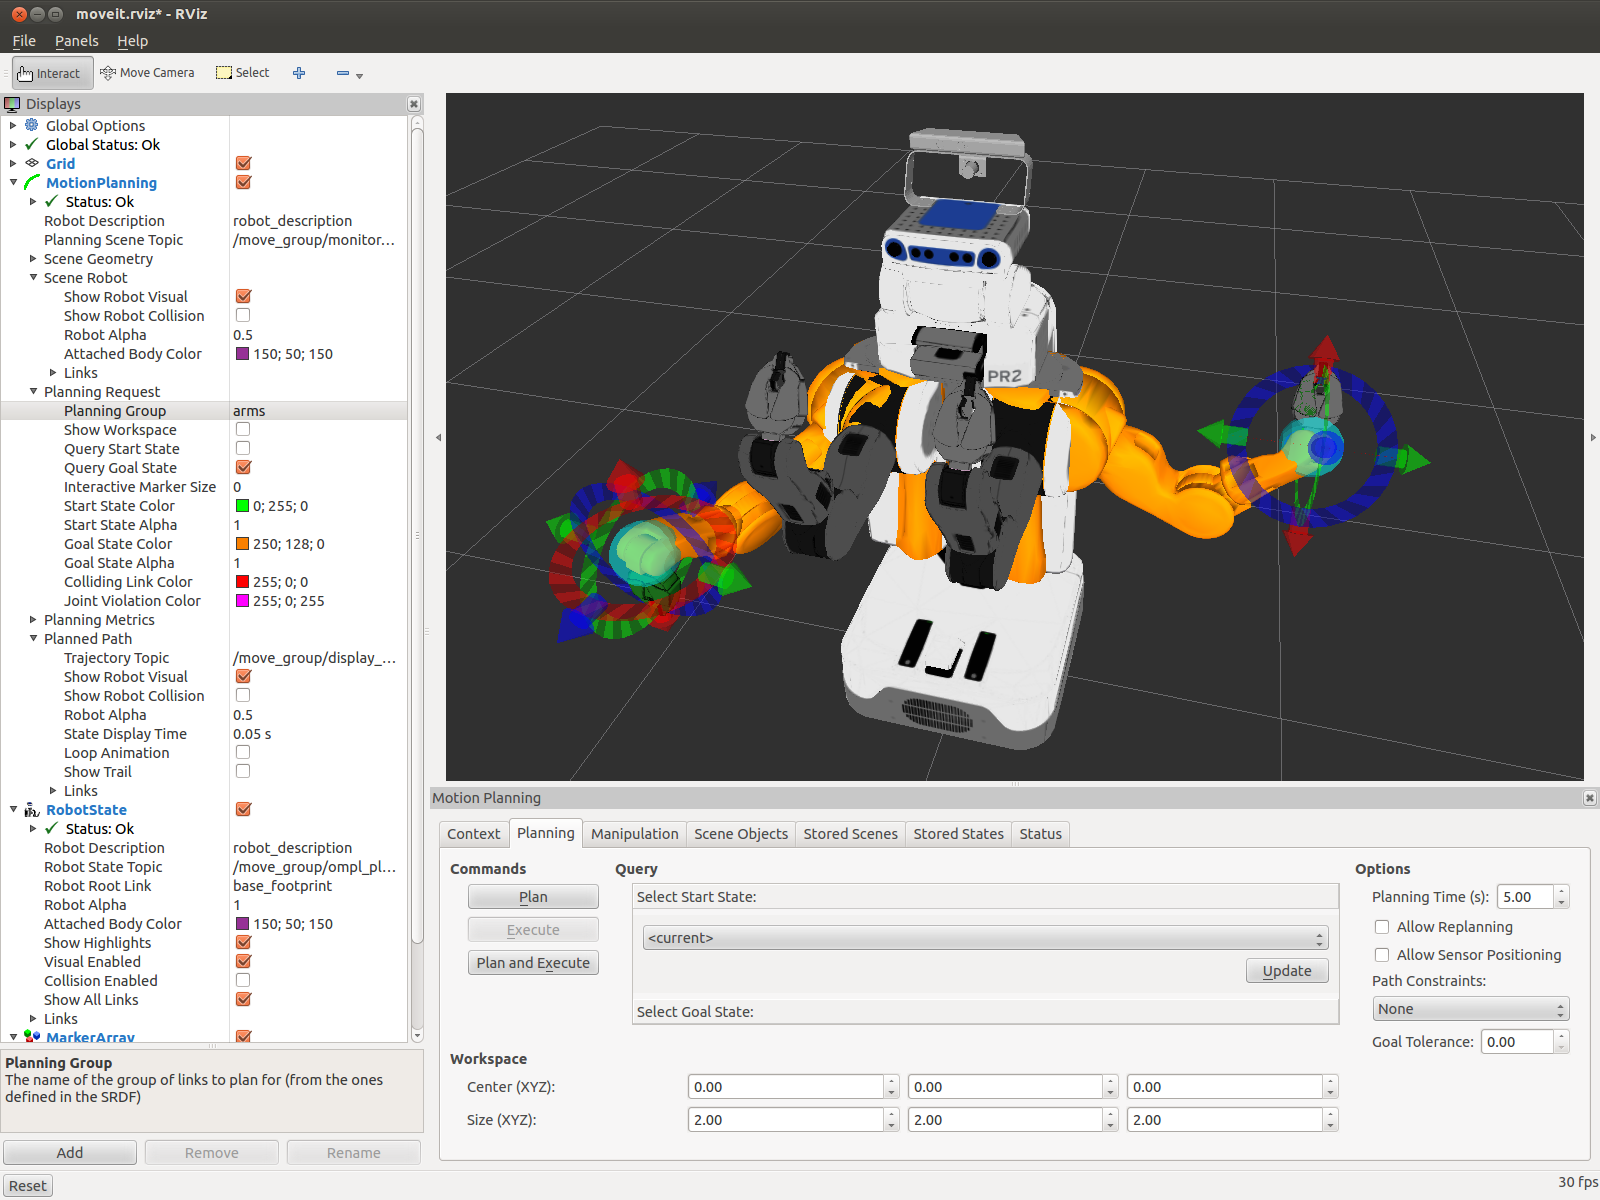
\includegraphics[width=3.4in]{images/rviz_motion_planning}
\caption{MoveIt! Motion Planning Visualization GUI with the PR2 planning with both arms to goal positions with interactive mouse-based tools}
\label{fig:motionrvizplugin}
\end{figure}

\begin{figure}[!t]
\centering
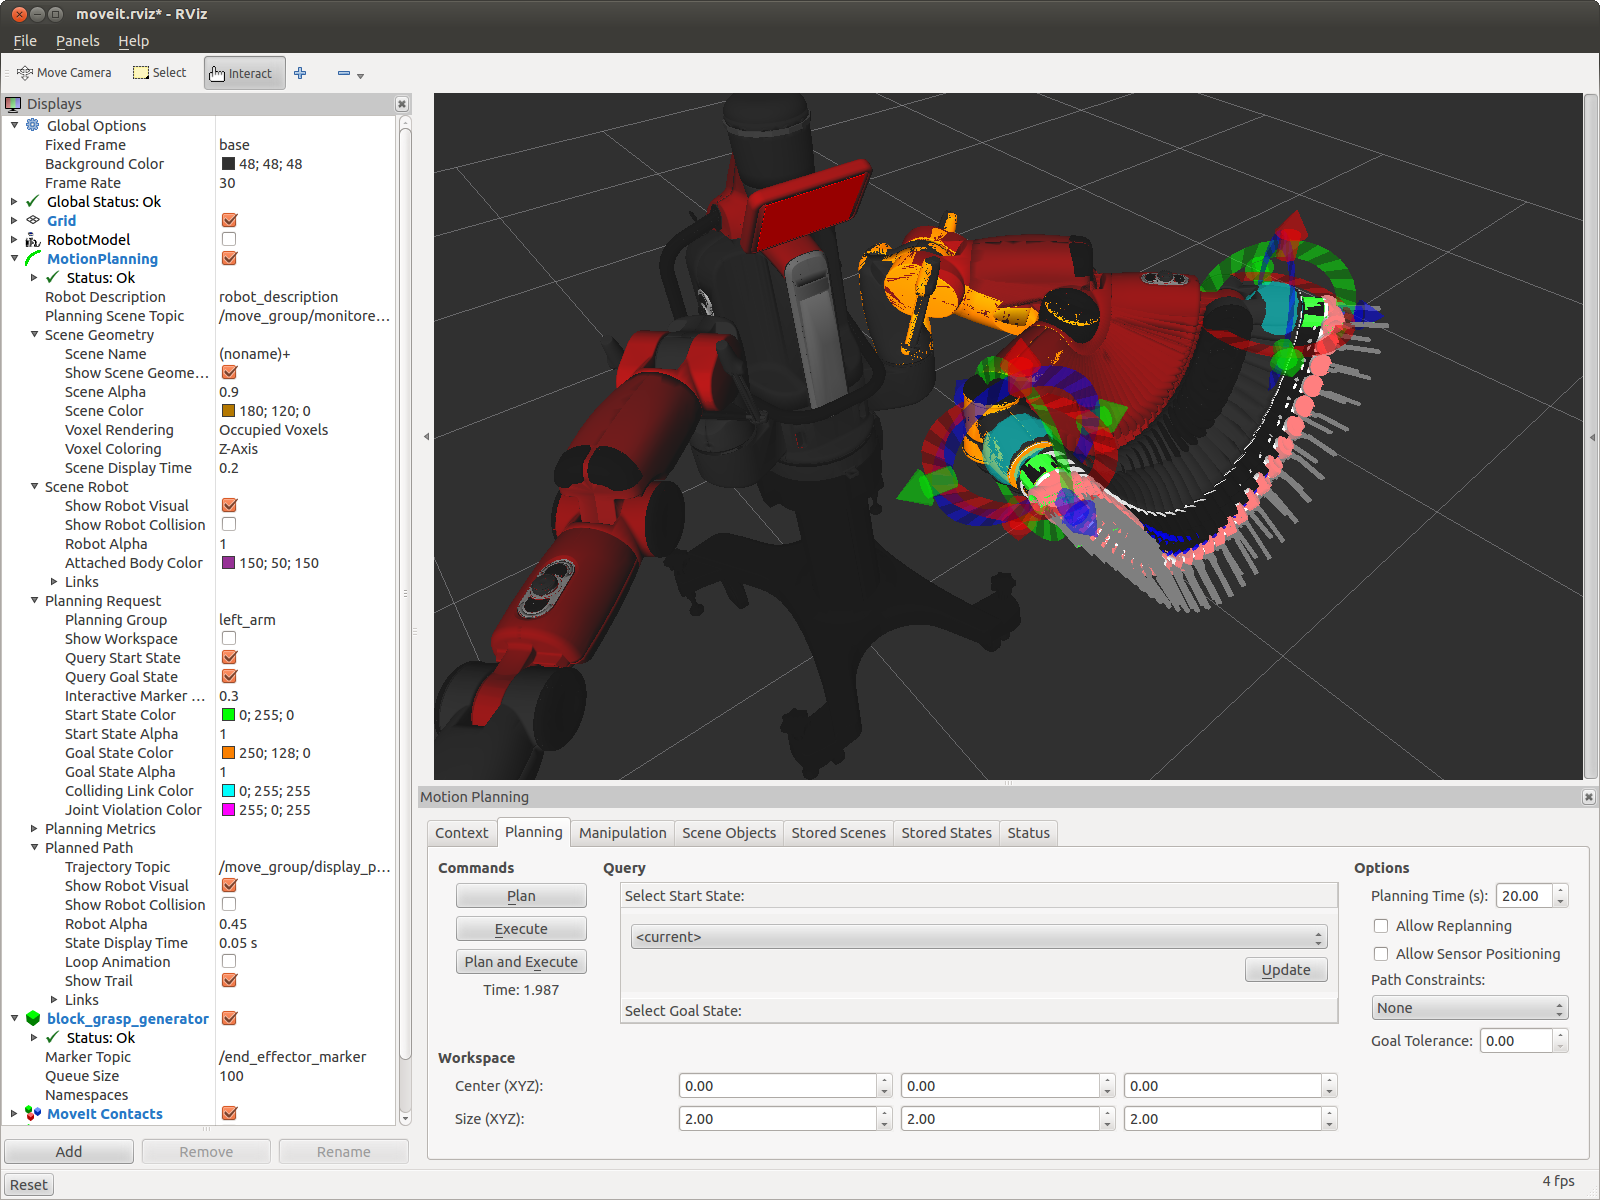
\includegraphics[width=3.4in]{images/motion_plan}
\caption{MoveIt! Motion Planning Visualization GUI with the Baxter robot visualizing steps of a motion plan}
\label{fig:motion_plan}	
\end{figure}

The MMPV provides a large number of features and visual tools for motion planning. Using MMPV, visualizations such as seen in Figure \ref{fig:motion_plan} are provided of:

\begin{itemize}
    \item Start and goal configurations of the robot for planning
    \item Current robot hardware configuration
    \item Animated planned path before executing
    \item Detected collisions
    \item Sensor data and recognized objects
    \item Pick and place data such as grasp positions
    \item Attached bodies such as manipulated objects
    \item Planning Metrics
\end{itemize}

Additionally, the MMPV contains many other non-visualization tools such as:
\begin{itemize}
    \item Connecting to a database of planning scenes
    \item Adjusting IK settings
    \item Changing the utilized planning algorithm
    \item Adjusting the workspace size
    \item Adjusting goal tolerance and planning time
    \item Tweaking manipulation plans
    \item Loading and moving collision objects
    \item Exporting/Importing scenes and states
    \item Viewing the status of MoveIt!
\end{itemize}

{\bf Hardware Configuration and Execution}: Once the user is comfortable with the basic tools and features provided by MoveIt!, the next step is to configure their robot's actual hardware actuators and control interfaces to accept trajectory commands from MoveIt!. This step is not as easy and requires some custom coding to account for the specifics of the robot hardware - the communication bus, real-time requirements, and control theory implementations. At the abstract level, all MoveIt! requires is that the robot hardware accepts a standard ROS trajectory message containing a discretized set of time-variant waypoints including desired positions, velocities, and accelerations.  

% ====================================================================
\subsection{Automatic configuration and optimization}

The size and complexity of a feature-rich MPF like MoveIt! requires many parameters and configurations of the software be automatically setup and tuned. MoveIt! accomplishes this in the 1) setup phase of a new robot, using the Setup Assistant, 2) during the runtime of the application, and 3) using benchmarking and parameter sweeping.

{\bf Self Collision Matrix}: The first step of the SA is the generation of a self-collision matrix for the robot that is used in all future planning to speed up collision checking. This collision matrix encodes pairs of links on a robot that never need to be checked for self-collision due to the kinematic infeasibility of there actually being a collision. Reasons for disabled collision checking between two links includes:
 
\begin{itemize}
    \item Links that can never intersect due to kinematics
    \item Adjacent links that are connected and so are by design in collision
    \item Links that are always in collision for any other reason including inaccuracies in the robot model and precision errors
\end{itemize}

This self-collision matrix is generated by running the robot through tens of thousands of random joint configurations and recording statistics of each link pair's collision frequency. The algorithm then creates a list of link pairs that have been determined to never need to be collision checked. This reduces future motion planning runtimes because it reduces the amount of required collision checks for every motion planning problem. The algorithm is incomplete because in very rare cases a pair of links will not be disabled for collision checking, but the result is a negligible amount of extra computation.

{\bf Configuration Files}: The other six steps of the SA all provide graphical front ends for the data required to populate the Semantic Robotic Description Format (SRDF) and other configuration files used by MoveIt!. The SRDF provides semantic meta data of the robot model useful to motion planning but not relevant to the URDF because it does not describe physical properties of the robot. The SRDF information includes which set of joints constitutes an arm and which set of links is considered part of the end effector. It is one of the main components that allows MoveIt! to be robot agnostic and to avoid dependencies on specific robots \cite{moveit}. Requiring the user to configure all the semantic information by hand in a text editor would be tedious and more difficult than using a GUI. The GUI populates the available options for each input field in list boxes and guides the user through filling in the necessary fields with buttons and graphical feedback.

The last step of the SA is to generate all launch scripts and configuration files. This step outputs to file the information collected from the user during the step-by-step user interface, as well as generates a series of default configuration and launch scripts that are automatically customized for the particular robot using the URDF and SRDF information. These defaults include velocity and acceleration limits for each joint, kinematic solvers for each planning group, available planning algorithms, and projection evaluators for planning. Default planning adapters are setup for pre- and post-processing of motion plans. Default benchmarking setups, controller and sensor manager scripts, and empty object databases are all generated using launch scripts, which essentially allow one to start different sets of MoveIt! functionality that are already put together. These defaults can later 
easily be modified by simply editing the text-based configuration files.

{\bf Automatic Runtime Tuning}: MoveIt! is designed to simplify solving planning problems by reducing the number of hard-coded parameters and so called ``magic numbers''. During runtime, MoveIt! is able to automatically choose good values for certain parameters to reduce the amount of expert domain knowledge required and make MoveIt! extensible to a larger set of problems. 

An example of automatic runtime tuning is the resolution in which collision checking is performed - it is defined as a fraction of the space extent. The space extent depends on the joint limits, the types of joints, and the planning groups being used. Another example is using projections to Euclidean spaces to estimate coverage during planning. By default in MoveIt!, the projects are computed randomly and their bounds are found by sampling. TODO: more details on this paragraph

{\bf Benchmarking}: The ability to configure and switch out different planning components is a powerful feature of MoveIt!, but its usefulness is limited without the ability to quantify the results of different approaches. Optimization criteria such as path length, planning time, smoothness, distance to nearest obstacle, and energy minimization need benchmarking tools to enable users and developers to find the best set of parameters and planning components for any given robotic application.

MoveIt! lowers the barrier to entry to benchmarking by providing a command line-based infrastructure and benchmarking configuration files that allows each benchmark to easily be setup for comparison against other algorithms and parameters \cite{cohen2012generic}. An additional GUI is currently in development that makes benchmarking even easier and reduces the learning curve to this feature set of MoveIt!.

Choosing the best combination of planning components and parameters for any particular robot and problem is a daunting task even for experts because of the number of choices that must be made\cite{cohen2012generic}. A common method to optimize an algorithms performance is to perform single and multivariable parameter sweeps during benchmarking. MoveIt! provides an interface for this in its benchmarking infrastructure by allowing a upper, lower, and increment search values to be provided by the user. Results can be output into generic formats for use in different plotting tools for analysis of which combination of parameters performed best.

% ====================================================================
\subsection{Easily customize components of the framework}
\label{subsec:extensiblity}

Out of the box, MoveIt! lowers the barrier to entry by not requiring users to provide their own implementation of any of the components in the motion planning framework. The default planning components are the aforementioned OMPL, FCL, and KDL. However, these default components are limiting to more advanced users who have their own application or research-specific needs to fulfill. 

\begin{figure}[!t]
\centering
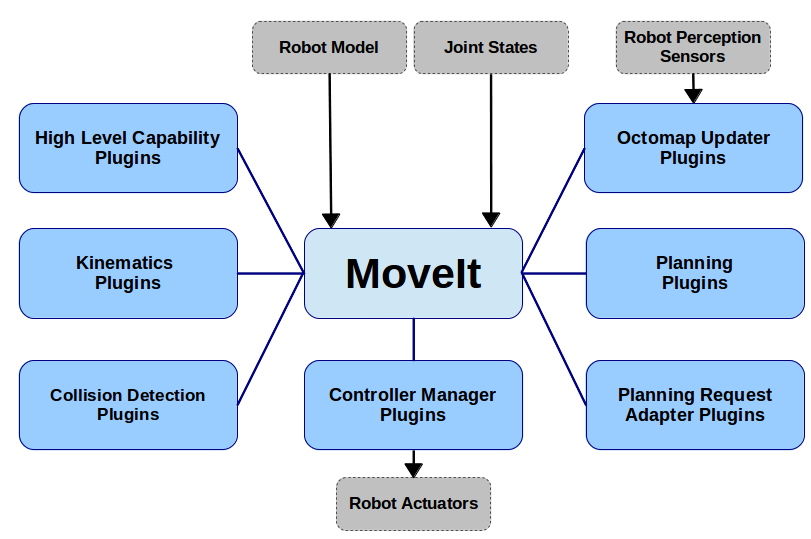
\includegraphics[width=3.4in]{images/moveit_plugins}
\caption{Available planning component plugins for easily extending the functionality of MoveIt!.}
\label{fig:moveit_plugins}
\end{figure}

{\bf Plugins}: MoveIt! is extensible by allowing its various planning components to be customized through a lightweight plugin interface. This is accomplished using C++ shared objects that are loaded at run time, reducing dependency complexities. This plugin-centric framework, as seen in Figure \ref{fig:moveit_plugins}, provides interfaces for forward and inverse kinematics, collision detection, planning, planning request adapters, controllers, octomap perception, and higher level capabilities. Almost all aspects of MoveIt!'s functionality can be extended using plugins.

A particular strong point of MoveIt!'s feature set is its kinematics plugins it can automatically generate using the input URDF. The default KDL plugin uses numerical techniques to convert from a Cartesian space to joint configuration space. A must faster solution can be achieved by utilizing OpenRave's IKFast \cite{ikfast} plugin that analytically solves the inverse kinematics problem. A combination of MoveIt! scripts and the IKFast Robot Kinematics Compiler can automatically generate the C++ code and plugin needed to increase the speed of motion planning solutions by up to 3 orders of magnitude \cite{ikfast}.

Essentially, MoveIt! provides a set of data sharing and synchronization tools, sharing between all planning components the robot's model and state. The extensibility of MoveIt!'s framework is greatly enhanced by not forcing users to use any particular algorithmic approach. 

{\bf High Level Interfaces}: High level custom task scripting is easily accomplished in MoveIt! with both a C++ and python interface that abstracts away most of the underlying mechanisms in MoveIt!. User who do not wish to bother with how the various low level planning components are operating can instead focus on the high level application tasks such as picking up an object and manipulating it. Python in particular is a very easy scripting language that enables powerful motion planning tasks to be accomplished with very little effort.

% ====================================================================
\subsection{Documentation and Community}

Though common place in open source software projects \cite{bruyninckx2001open}, it should be mentioned for completeness that MoveIt! addressed the \textit{entry barrier design principle} of \textit{documentation} by providing extensive wiki pages, a mailing list for questions, and a issue tracker for bug reports and feature requests.

% ====================================================================
% ====================================================================
% Section
% ====================================================================
% ====================================================================
\section{Results}
\label{sec::results}

The success of MoveIt!'s efforts to lower its barrier of entry to new users through the application of the barrier to entry principles is quantified in the following. Its adoption rate, community activity, contributors, and results from a user survey are used as indicators of its progress.

\subsection{Statistics}
\label{sec::statistics}

MoveIt! was officially alpha released on May 6th, 2013 - 183 days as of this writing. One method to quantify its popularity is by the total number of pre-build binary and source code installations that have been performed. Though not exactly representative of this data, MoveIt!'s website has an ``Installation'' page that has received 7,688 page views since being launched \cite{moveit}, of which a large fraction of that number can be assumed to represent unique installations. 

There are currently 177 users on the MoveIt! mailing list as shown over time in Figure \ref{fig:membership_plot}. The posting activity of the mailing list over time is also shown in Figure \ref{fig:membership_plot}.

\begin{figure}[!t]
\centering
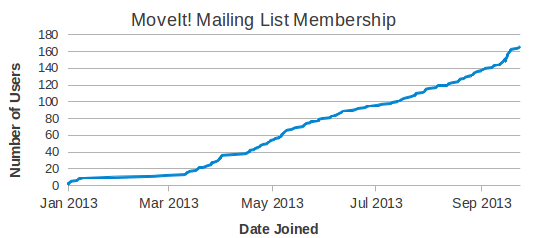
\includegraphics[width=3.4in]{images/membership_plot}
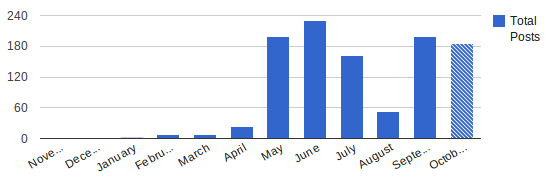
\includegraphics[width=3.4in]{images/mailing_list}
\caption{MoveIt! Mailing List Statistics. MoveIt! was alpha released in May}
\label{fig:membership_plot}
\end{figure}

There have been a total of 48 contributors to the MoveIt! code base since its initial development began in 2011. The total number of contributors over time is shown in Figure \ref{fig:contributors}. According to statistics gathered by Ohloh, MoveIt! is ``one the largest open-source teams in the world and is in the top 2\% of all project teams on Ohloh'' \cite{ohloh}.

\begin{figure}[!t]
\centering
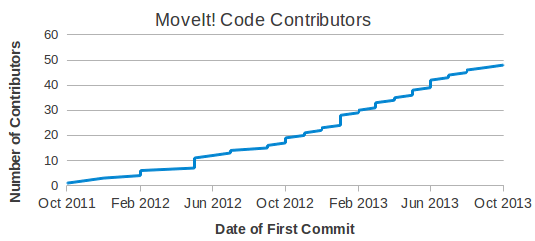
\includegraphics[width=3.4in]{images/moveit_contributors}
\caption{MoveIt! Source Repository Statistics}
\label{fig:contributors}
\end{figure}

\subsection{Survey}
\label{sec::survey}

\begin{figure}[!t]
\centering
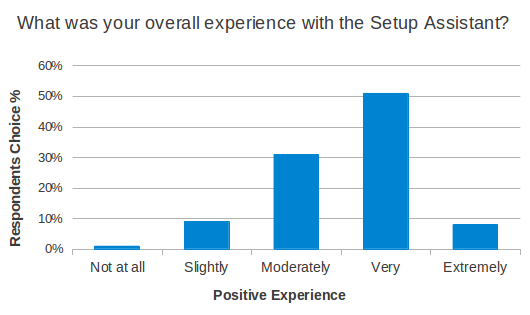
\includegraphics[width=3.4in]{images/setup_assistant_positive}
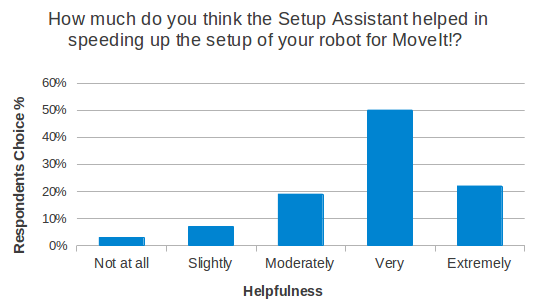
\includegraphics[width=3.4in]{images/sa_speedup}
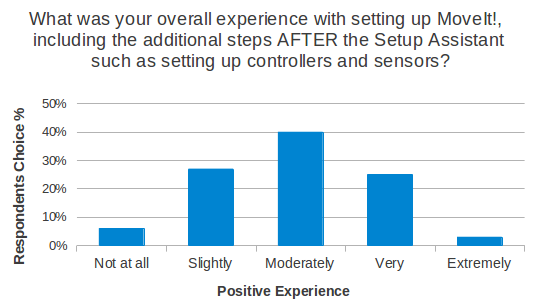
\includegraphics[width=3.4in]{images/moveit_after_sa}
\caption{Survey data of 105 respondents on the MoveIt! and ROS mailing lists.}
\label{fig:setup_assistant_positive}
\end{figure} 

A survey on user's experience with MoveIt! was administered over the MoveIt! and ROS mailing lists. There were a total of 105 respondents, TODO talk about their demographics. Relevant results are shown in Figure \ref{fig:setup_assistant_positive}. 

Respondents were asked to rate their overall experience with using the MoveIt! Setup Assistant, and asked how much the SA helped in speeding up setup of a robot in MoveIt!. For both questions, ninety percent had moderate to extremely good experiences with the SA, and for both questions over half rated their experience 'very good'. 

Respondents were then asked what their overall experience was with setting up and configuring MoveIt!, including any additional steps they had to take after the SA such as setting up controllers and sensors. In this question, the results were less positive. Forty percent had a moderately positive experience, but only 28\% had a 'very' or 'extremely' positive experience. 

An additional question asked respondents 'how many minutes would you estimate you spent going from a URDF to solving motion plans using the MoveIt! Motion Planning Visualizer?'. The responses to this question had a large amount of variance with the mean time taking users 1.5 hours with a standard deviation of 2 hours.



% ====================================================================
% ====================================================================
% Section
% ====================================================================
% ====================================================================
\section{Discussion}
\label{sec::discussion}

\subsection{MoveIt! Setup}
\label{sec::moveit_discussion}

We believe the barrier to entry for MoveIt! is easier than most, if not all, open source robotics software available today as discussed in Section \ref{sec::existing}. As a result MoveIt! has quickly become popular in the robotics community as a powerful motion planning framework that is extensible to most user's needs for their robot application. The adoption rate of MoveIt! since its official release less than half a year ago has been very positive in comparison to the size of the world wide robotics community. With 177 users on the mailing list since MoveIt!'s release, a new member has joined the project at a rate of nearly once per day. Though a very rough estimate, it can additionally be approximated that MoveIt! has been installed seven thousand times, or 38 times per day since its release. These numbers indicate a healthy usage and popularity of this open source software project.

Community effort to improve MoveIt! has been better than expected with a total of 48 code contributors during MoveIt!'s existence. Ohloh's ranking of MoveIt! as one of the largest open source teams in the world confirms our belief that by making complex software more accessible, more developers will be able to report and fix issues. 

Still, the setup and configuration process has room for improvement as indicated by the survey's TODO. 

It is important to emphasize the effect of a quick \textit{Getting Started} demo on a new user unaccustomed to MoveIt! or motion planning in general. The positive reinforcement of a quick initial success encourages the novice to continue to use the software and enables them to begin going deeper into the functionality and code base. If the entry barrier is too high, that is to say if it is too complex and error-prone, a new user will likely give up and turn to other frameworks or custom solutions. Attempting to blindly fix software that a new user has not had any success with is a very difficult task.

Creating the robot model itself is a difficult task that typically requires a lot of trial and error in configuring the links and joints properly. This process could be improved by a better GUI for making arbitrary robot models. TODO elaborate 

Setting up the hardware controllers can also be a difficult task for non-experts and the MoveIt! setup process does not document and provide example code as well as it could. It is likely this step will continue to require some custom coding to account for arbitrary hardware interfaces and communication methods, but based on the feedback we have received from actual users, this is certainly an area of improvement. 



Finally, although MoveIt! is very extensible with its plugin-based architecture, modifying the actual code base of MoveIt! can be intimidating due to its large size. MoveIt! contains over 170 thousand lines of code across all its various packages. Due to the need for computational speed and power, the layout of the code can sometimes seem complicated and too abstracted. Finally, over half of the code base has been created by a single developer, so readability has not been the highest objective. 

\subsection{Robotic Software}
\label{sec::robotic_discussion}

The techniques utilized in the development of MoveIt! can easily be applied to robotics software in general. Almost all robotics software requires customizations specific to a particular hardware and kinematic configuration. Reducing the difficulty of performing these customizations should be the goal of robotic software engineers who desire to create useful tools for a large audience. 

For example, in perception applications such as visual servoing, frame transforms must be specified of the location of the camera to the rest of the robot's geometry. This is often a difficult and tedious task CITE. Automating the calibration of these transforms lowers the barrier of entry to new users to robotic vision software and makes the vision software useful to more users.

Creating a GUI such as the Setup Assistant is a time consuming process that many robotics developers avoid in favor of manual or command-line based configuration. As discussed in the introduction, we believe that the trade off in the time invested is worthwhile for the higher adoption rates and creation of a larger community willing to contribute to the software's development. It is understandable that when robotics research is the priority, spending time on tangential aspects of the project such as GUIs and configuration tools can be less important to the researcher. Still, we would like to encourage researchers and developers alike to, when possible, spend the extra time making their work reusable by taking into consideration the barriers to entry that other users might encounter. Too often, software is touted as ``open source'' when its usefulness is in actuality severely limited by the difficulties encountered in applying it to other projects by other users. By sharing accessible open source robotics 
software, the progress of robotic technology is accelerated and the robotics community on the whole benefits.

TODO: more about how these results can be generalized and standardized

% ====================================================================
% ====================================================================
% Section
% ====================================================================
% ====================================================================
\section{Conclusion}
\label{sec::conclusion}

Beyond the usual considerations in building successful robotics software, an open source project that desires to maintain an active user base needs to take into account the barrier of entry to new users. As the algorithms become more complicated and the number of planning components and size of the code base increases, configuring an arbitrary robot to utilize robotic software becomes a daunting task requiring domain-specific expertise in a very large breadth of theory and implementation. To account for this, quick and easy initial configuration, with partially automated optimization, and easily extensible components for future customization are becoming a greater necessity in motion planning and robotic software engineering in general. 

% ====================================================================
% ====================================================================
% Section
% ====================================================================
% ====================================================================
\section*{Acknowledgments}
The authors would acknowledge E. Gil Jones as the initiator and Matthew Klingensmith as the implementor of the Arm Navigation Setup Wizard, the inspiration for the MoveIt! Setup Assistant.

TODO: references lack details such as journal title etc. 
TODO: ''Where available, URLs for the references have been provided.''
% references section
\bibliographystyle{IEEEtran}
% argument is your BibTeX string definitions and bibliography database(s)
\bibliography{IEEEabrv,moveit_setup_bibliography}


% biography section
\begin{IEEEbiography}[{coleman}]{David Coleman}, M.S., 2013, is a Ph.D. candidate in Computer Science at the University of Colorado. He obtained his B.S. in Mechanical Engineering at the Georgia Tech and Masters in C.S. at CU Boulder. David's research interests include robotic manipulation, motion planning, and controls. He is one of the main developers of MoveIt!, creating the MoveIt! Setup Assistant while interning at Willow Garage continuing development at the Open Source Robotics Foundation and with his regular research.
\end{IEEEbiography}

\begin{IEEEbiography}[{}]{Ioan Sucan}, lorem
\end{IEEEbiography}

\begin{IEEEbiography}[{}]{Sachin Chitta}, lorem
\end{IEEEbiography}

\begin{IEEEbiography}[{nikolauscorrell}]{Nikolaus Correll}, M.S., 2003, Ph.D., 2007, is an Assistant Professor in Computer Science at the University of Colorado. He obtained his Master's degree in Electrical Engineering from ETH Z\"urich, a Ph.D. in Computer Science from EPFL and worked as a post-doc at MIT CSAIL. Nikolaus's research interests are multi-robot and swarming systems. He teaches ``Introduction to Robotics'' and ``Advanced Robotics'' to third- and fourth-year students.
\end{IEEEbiography}


% insert where needed to balance the two columns on the last page with
% biographies

% You can push biographies down or up by placing
% a \vfill before or after them. The appropriate
% use of \vfill depends on what kind of text is
% on the last page and whether or not the columns
% are being equalized.

\vfill

% Can be used to pull up biographies so that the bottom of the last one
% is flush with the other column.
%\enlargethispage{-5in}

% that's all folks
\end{document}
